\documentclass[a4paper]{article} 

\usepackage[frenchb]{babel}
\usepackage[utf8x]{inputenc}
\usepackage[T1]{fontenc}
\usepackage{minted}
\usepackage{graphicx}
\usepackage{pifont}
%\usepackage[nochapters]{classicthesis} 
%
\usepackage[a4paper,top=3cm,bottom=2cm,left=3cm,right=3cm,marginparwidth=1.75cm]{geometry}
\setlength{\parskip}{.5em}

%

\title{Projet Programmation Systeme}
\author{Pierre CHAUVEAU, Remi BRISSET, Francois AUDOY}
\date{\today} % no date

\graphicspath{{screenRapport/}} 

\begin{document}

\maketitle


\begin{abstract}
  ici on fait l'introduction / résumé du projet
\end {abstract}

\part{Sauvegarde et chargemement des cartes}

test des accents déjà où ça
Ecrire ici le contenue de la première partie
\section{Sauvegarde}
Idem

\section{Chargement}
Idem

\section{Utilitaire de manipulation de carte}
Pour nous assister dans nos tests, nous avons implémenté un executable readMap affichant sur la sortie standard le contenu d'un \emph{file} issu d'une map sauvegardée.
Exemple d'utilisation:
petite image des familles 

\subsection{Une erreur surprenante}
L'utilisation de xargs nous a posé dans un premier temps beaucoup de soucis. En effet pour une raison qui nous est toujours inconnue l'odre des premier arguments change lors de l'utilisation de xargs. C'est grâce à l'utilisation de notre fonction de test % \begin{minted}[c] void print\_args(int argc, char** argv);  \end{minted}
\\
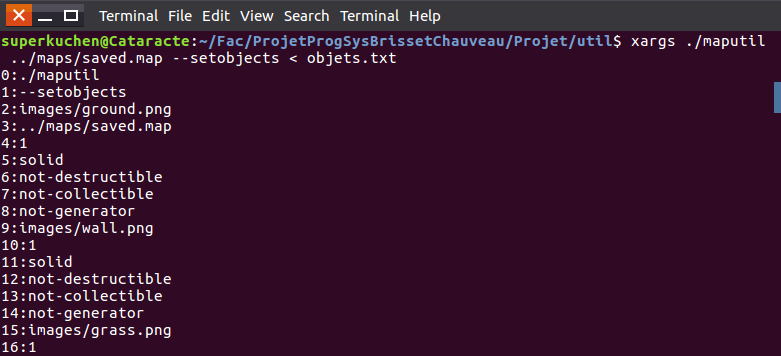
\includegraphics[scale=0.5]{erreurArgs.png}

\part{Gestion des temporisateurs}
Idem

\section{Choix d'implémentation}
idem

\section{autre sous section}
ide

\end{document}
